\section{Gitter}

Fælles for alle 3 systemer er kølegitteret af aluminium, der er i kontakt med processoren. 
I simple systemer udgør den den eneste part i kølesystemet og kan selvfølgelig bestå af andre materialer end Aluminium. 
Men i rapporten her vil aluminum blive brugt

Kølegitteret udnytter overfladeareal til at bortlede varme ved konvektion fra et fast materiale(aluminium) til et fluid(atmosfærisk luft) .
Således vil der være to termiske modstande, navnlig varmeledningsmodstand og varmeovergangsmodstand.

En hyppig forekommende struktur i et kølegitter er ribbe, der giver en naturlig strømning af den varme luft bort fra kølegitteret. Hvor kun er termodynamiske kræfter har indflyldelse på strømningen. Men strømningen foregår foregår imellem to kanalvægge. 

Der præsenteres her en oversigt over de værdier der bruges i udregningerne: 

Der beregnes varmestrøm for konvektion og for stråling.

Tallene for ovenstående kølegitter er importeret fra en partfil i Solidworks. %Kanalen for strømningen af luft der regnes for er d(1mm) bred og den hydraulisk diameter regnes som værende en snæver kanal, hvor L=2*a

H = 20 mm, $b = 25,5 mm$, $d  =1 mm$ ,Areal $A_t = 93733.73 mm^2$ , $A_{lam}= 500 mm^2$  \\ 
$ Massen m = 31,58 gr.$ \\
Varmekonduktiviten for aluminium, $\lambda_{al} = 228$ \\  
Lameltykkelsen $\delta = 0.5 mm.$  \\\
Den specifikke varmekapacitet $c\_p = 1.008$ \\
Strømningshastighed lodret, i lamellets længde på $c = 0.001$ \\



For at udregne varmestrømmen $\phi$  bruges udtrykket \\ $\Phi = \alpha * A* (t\_{fl}-t\_v$ \\  også kendt som Newtons ligning. \\ 
Hvoraf varmekonduktiviteten $\alpha$ er fundet ved tabel opslag $\alpha = 21.8$ \\
Kinematisk viskositet er: $18.88$ og dynamisk viskositet = $16.92$  \\
Volumenudvidelseskoefficienten $\beta_luft = 3,2$ \\
 
Varmeledningsmodstanden : $R_l = \frac{\delta}{\lambda_{al}*A_{lam}} = 4.281$ \\
Varmeovergangsmodstanden : $R_o = \frac{1}{\alpha_{tl}*A_{lam}} = 89.394$ \\

Total termisk modstand er $R_{tot} = R_l + R_o = 92.225$ \\

\section{Beregninger}

Varmestrømmen $\phi$ udregnes ved ligningen Nu = $\frac{\alpha}*{\lambda}$ \\
Nu er Nusselts tal og findes herunder ved at udregne Reynolds(Re) og Prandtls(pr) tal.


Strømningsforholdende for luft(fluiden) imellem lammelerne i gitteret er fri indvendig strømning, idet, lamellerne kan ses som kanalvægge og udgangen i en antaget lodret given retning er smal og bred. med 3 åbne sider og derved tillader en fri udvikling af strømningen. Hvor den dydrauliske diameter er i brug og sættes lig med afstanden imellem 2 givene lameller. $\approx 0.5 mm$

Reference temperaturen udregnes til : 
\\$t_{film} = \frac{{t_{lam}}+t_{fluid}}{2} => t_{film}=30$
\\Grasshofs tal Gr = $\frac{g*L^3*\beta*{\Delta\,t}}{\upsilon\,^2} = 8,771*10^4$
\\Prandtls tal Pl(opslag) => $Pr=0.69$


Der antages lodret  strømning af luften og Reynold tal undersøges for at få et hit om strømningsformen\\

$Re = \frac{c_{luft}*L_{hyd}}{\upsilon} = 2.648*10^{-5}$
%$ Ra = Gr*Pr = 6.052*10^4$ => \\ 
Hvilket indikerer laminar strømning over hele længden af et lamel. 
Hvorfor strømningen ikke undersøges yderligere, idet Re er $10^9$ mindre, end den forventede kritiske værdi for turbulent strømning.

Hastghedsprofilet hvorved den opvarmede luft stiger til vejr er udregnet til: 
$0.05*Re*L_{hd} = 0.001 $

Hvilket medfører at Nusselts tal kan udregnes som \\ 
$Nu = 3,66+ \frac{0.0668*Re*Pr*\frac{D}{L_{lam}}}{1+0.004*()\frac{D}{L_{lam}}k *Re*Pr})^{2/3} = 3.661$


%Den kritisk værdi findes da ved: $Nu_m = C*Ra^4$

og $ \Phi = \alpha*A(t_{fl}-t_v =>2.597*10^6 W $\\ 
justeret til milimeter ved udtrykket: $\frac{\Phi = \alpha*A*(t_{fl}-t_v}{10^6} =>0.75 W$

samtlige lammeler afgiver da $0,75 w* 40 \approx 30 W$ i varmestrøm til luften der passerer. 

\begin{figure}
	\centering
	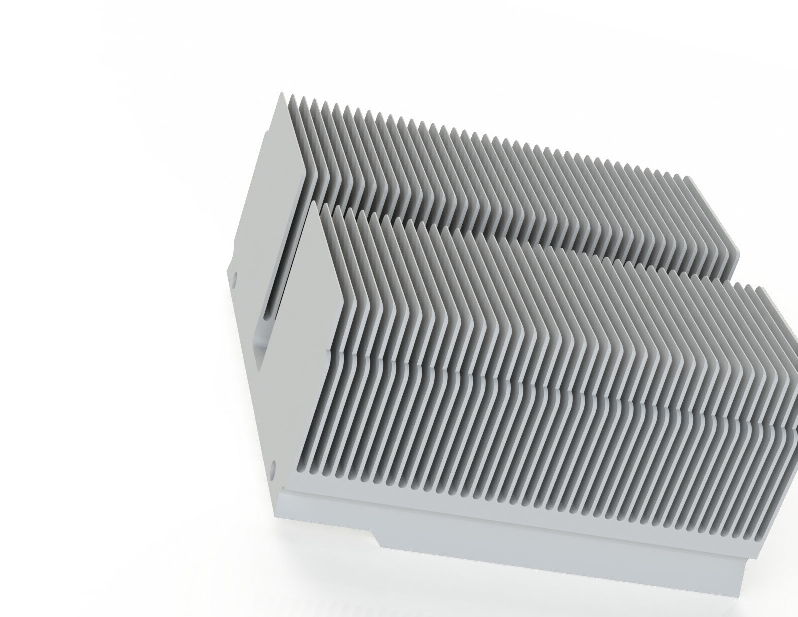
\includegraphics[width=0.7\linewidth]{billeder/heatsink1}
	\caption{Eksempel på kølegitter, Fra grabcad.com - bruger: Fernando}
	\label{fig:heatsink1}
\end{figure}


\begin{figure}
	\centering
	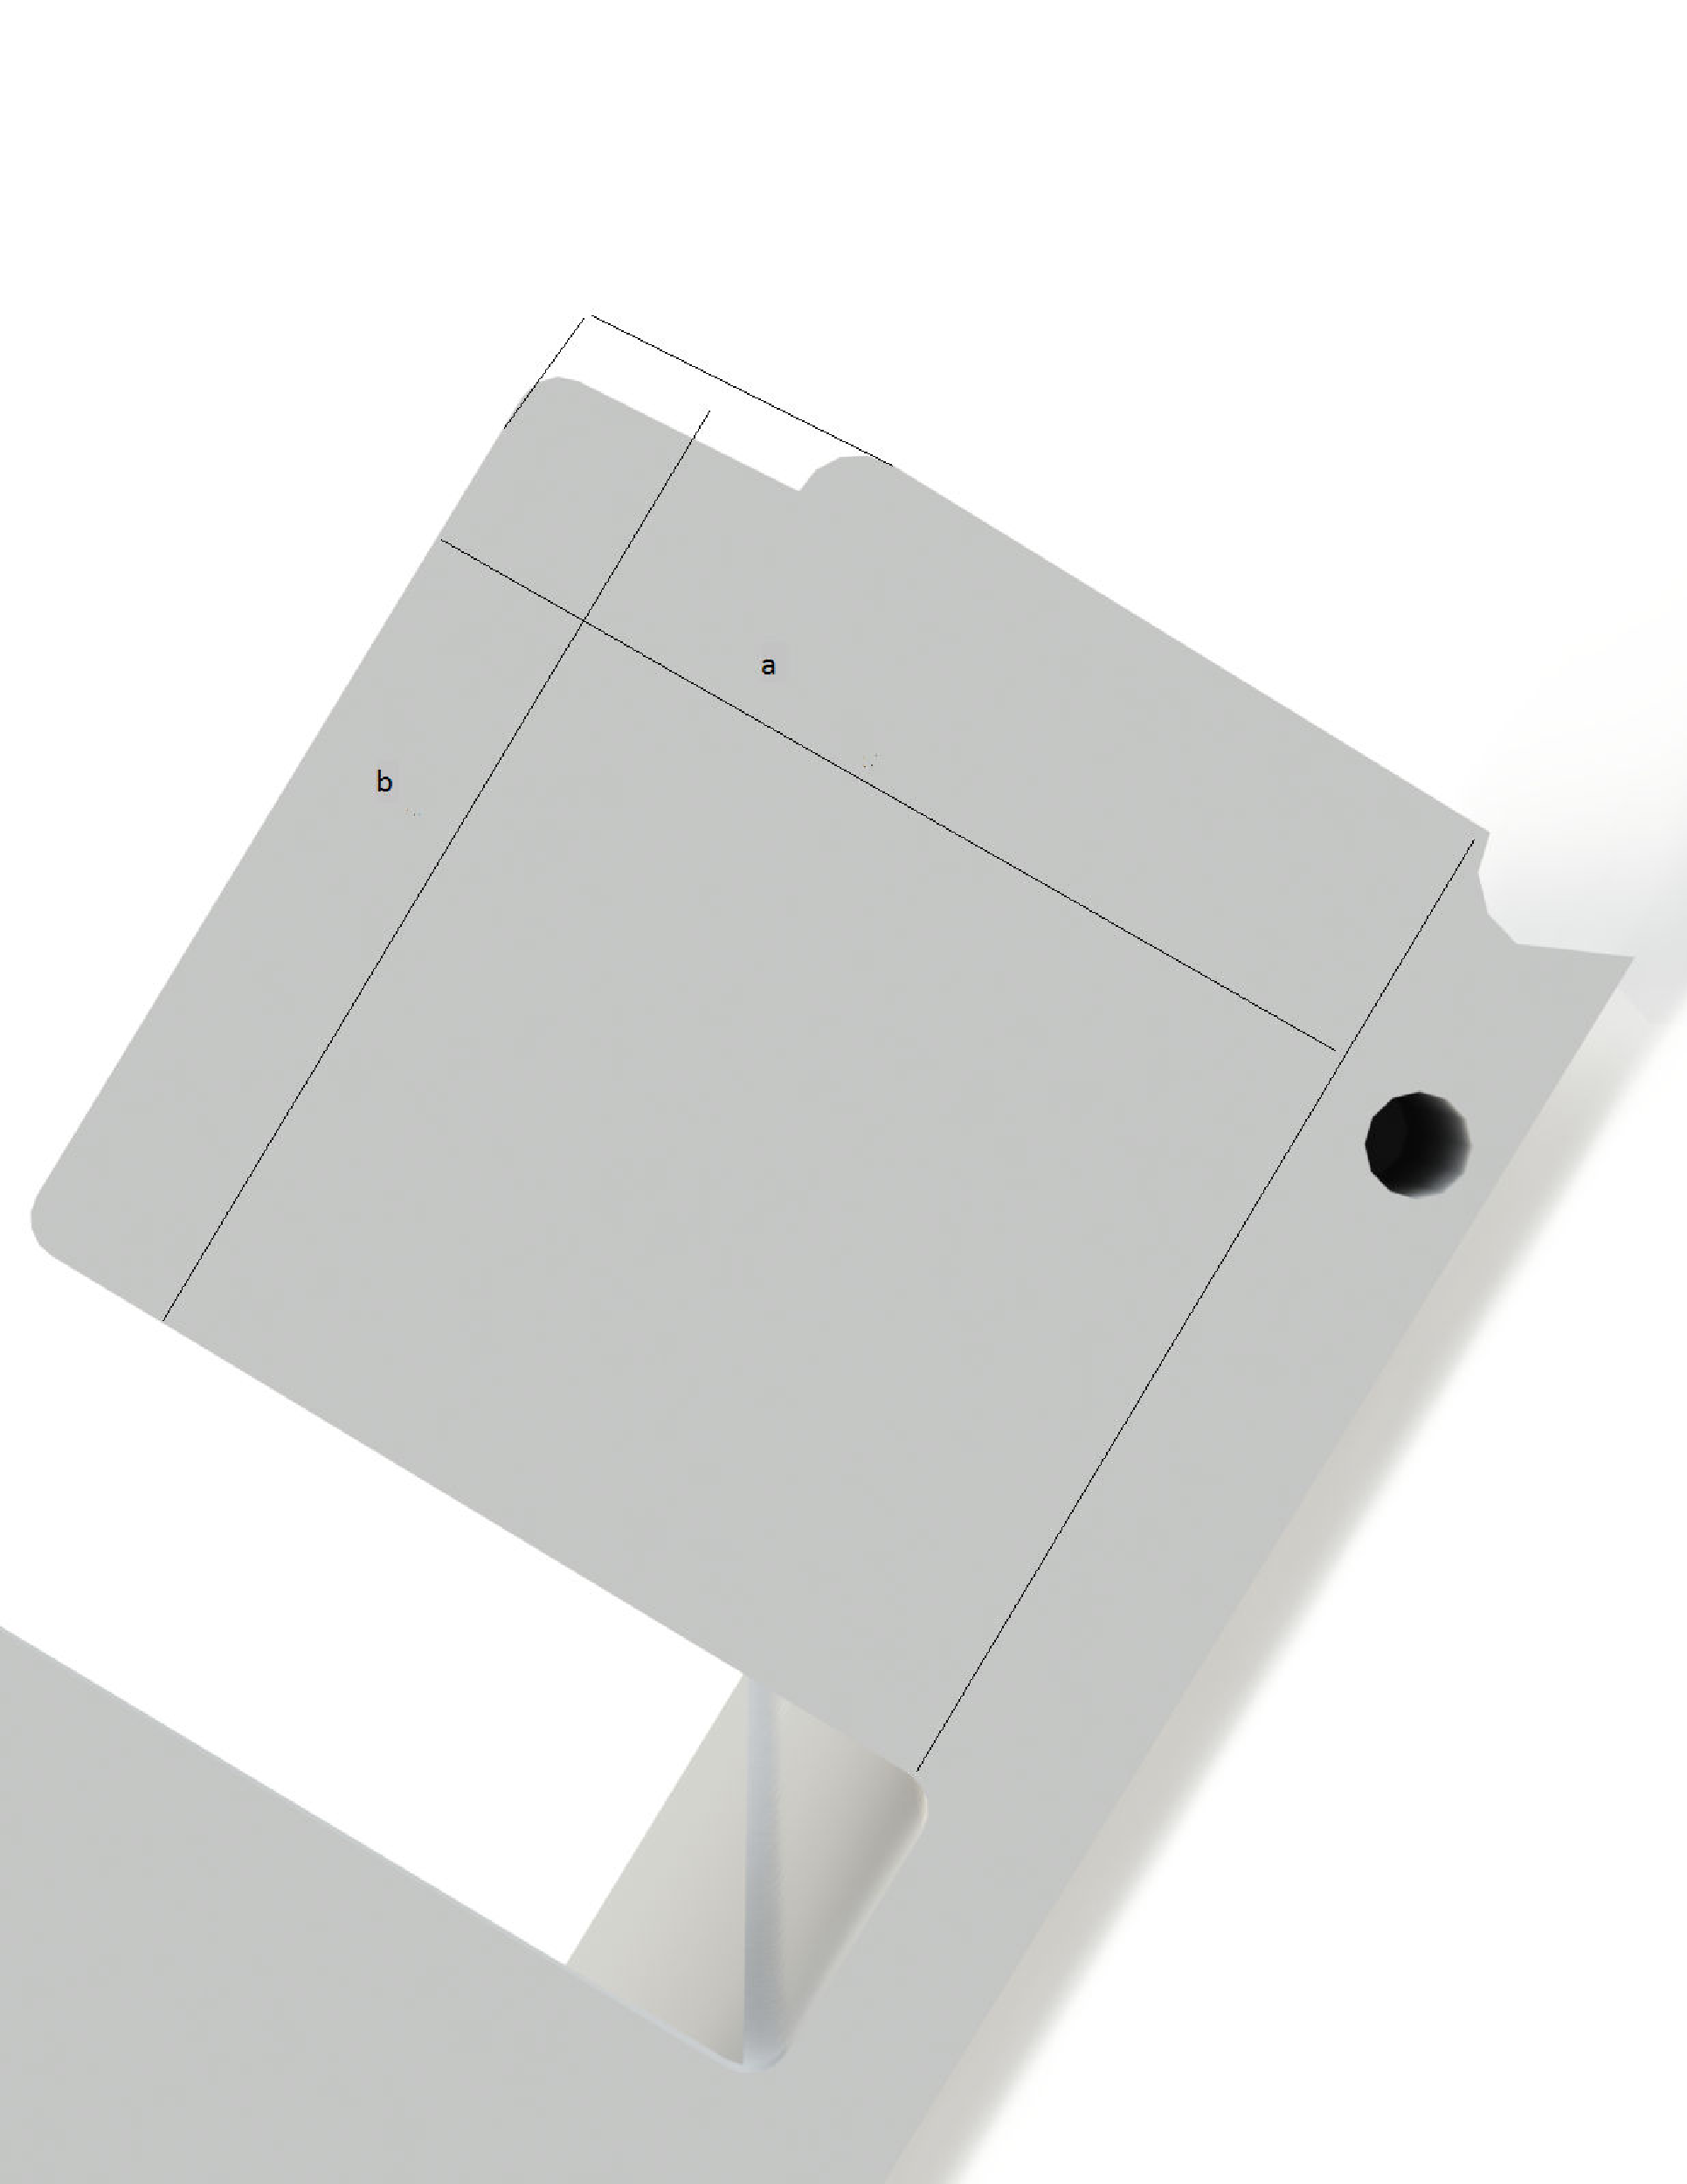
\includegraphics[width=0.7\linewidth]{billeder/lamel}
	\caption{Lamel. genstand for vore termdynamiske undersøgelser.Fra grabcad.com - bruger: Fernando}
	\label{fig:lamel}
\end{figure}
